% Options for packages loaded elsewhere
\PassOptionsToPackage{unicode}{hyperref}
\PassOptionsToPackage{hyphens}{url}
%
\documentclass[
]{article}
\usepackage{amsmath,amssymb}
\usepackage{iftex}
\ifPDFTeX
  \usepackage[T1]{fontenc}
  \usepackage[utf8]{inputenc}
  \usepackage{textcomp} % provide euro and other symbols
\else % if luatex or xetex
  \usepackage{unicode-math} % this also loads fontspec
  \defaultfontfeatures{Scale=MatchLowercase}
  \defaultfontfeatures[\rmfamily]{Ligatures=TeX,Scale=1}
\fi
\usepackage{lmodern}
\ifPDFTeX\else
  % xetex/luatex font selection
\fi
% Use upquote if available, for straight quotes in verbatim environments
\IfFileExists{upquote.sty}{\usepackage{upquote}}{}
\IfFileExists{microtype.sty}{% use microtype if available
  \usepackage[]{microtype}
  \UseMicrotypeSet[protrusion]{basicmath} % disable protrusion for tt fonts
}{}
\makeatletter
\@ifundefined{KOMAClassName}{% if non-KOMA class
  \IfFileExists{parskip.sty}{%
    \usepackage{parskip}
  }{% else
    \setlength{\parindent}{0pt}
    \setlength{\parskip}{6pt plus 2pt minus 1pt}}
}{% if KOMA class
  \KOMAoptions{parskip=half}}
\makeatother
\usepackage{xcolor}
\usepackage[margin=1in]{geometry}
\usepackage{color}
\usepackage{fancyvrb}
\newcommand{\VerbBar}{|}
\newcommand{\VERB}{\Verb[commandchars=\\\{\}]}
\DefineVerbatimEnvironment{Highlighting}{Verbatim}{commandchars=\\\{\}}
% Add ',fontsize=\small' for more characters per line
\usepackage{framed}
\definecolor{shadecolor}{RGB}{248,248,248}
\newenvironment{Shaded}{\begin{snugshade}}{\end{snugshade}}
\newcommand{\AlertTok}[1]{\textcolor[rgb]{0.94,0.16,0.16}{#1}}
\newcommand{\AnnotationTok}[1]{\textcolor[rgb]{0.56,0.35,0.01}{\textbf{\textit{#1}}}}
\newcommand{\AttributeTok}[1]{\textcolor[rgb]{0.13,0.29,0.53}{#1}}
\newcommand{\BaseNTok}[1]{\textcolor[rgb]{0.00,0.00,0.81}{#1}}
\newcommand{\BuiltInTok}[1]{#1}
\newcommand{\CharTok}[1]{\textcolor[rgb]{0.31,0.60,0.02}{#1}}
\newcommand{\CommentTok}[1]{\textcolor[rgb]{0.56,0.35,0.01}{\textit{#1}}}
\newcommand{\CommentVarTok}[1]{\textcolor[rgb]{0.56,0.35,0.01}{\textbf{\textit{#1}}}}
\newcommand{\ConstantTok}[1]{\textcolor[rgb]{0.56,0.35,0.01}{#1}}
\newcommand{\ControlFlowTok}[1]{\textcolor[rgb]{0.13,0.29,0.53}{\textbf{#1}}}
\newcommand{\DataTypeTok}[1]{\textcolor[rgb]{0.13,0.29,0.53}{#1}}
\newcommand{\DecValTok}[1]{\textcolor[rgb]{0.00,0.00,0.81}{#1}}
\newcommand{\DocumentationTok}[1]{\textcolor[rgb]{0.56,0.35,0.01}{\textbf{\textit{#1}}}}
\newcommand{\ErrorTok}[1]{\textcolor[rgb]{0.64,0.00,0.00}{\textbf{#1}}}
\newcommand{\ExtensionTok}[1]{#1}
\newcommand{\FloatTok}[1]{\textcolor[rgb]{0.00,0.00,0.81}{#1}}
\newcommand{\FunctionTok}[1]{\textcolor[rgb]{0.13,0.29,0.53}{\textbf{#1}}}
\newcommand{\ImportTok}[1]{#1}
\newcommand{\InformationTok}[1]{\textcolor[rgb]{0.56,0.35,0.01}{\textbf{\textit{#1}}}}
\newcommand{\KeywordTok}[1]{\textcolor[rgb]{0.13,0.29,0.53}{\textbf{#1}}}
\newcommand{\NormalTok}[1]{#1}
\newcommand{\OperatorTok}[1]{\textcolor[rgb]{0.81,0.36,0.00}{\textbf{#1}}}
\newcommand{\OtherTok}[1]{\textcolor[rgb]{0.56,0.35,0.01}{#1}}
\newcommand{\PreprocessorTok}[1]{\textcolor[rgb]{0.56,0.35,0.01}{\textit{#1}}}
\newcommand{\RegionMarkerTok}[1]{#1}
\newcommand{\SpecialCharTok}[1]{\textcolor[rgb]{0.81,0.36,0.00}{\textbf{#1}}}
\newcommand{\SpecialStringTok}[1]{\textcolor[rgb]{0.31,0.60,0.02}{#1}}
\newcommand{\StringTok}[1]{\textcolor[rgb]{0.31,0.60,0.02}{#1}}
\newcommand{\VariableTok}[1]{\textcolor[rgb]{0.00,0.00,0.00}{#1}}
\newcommand{\VerbatimStringTok}[1]{\textcolor[rgb]{0.31,0.60,0.02}{#1}}
\newcommand{\WarningTok}[1]{\textcolor[rgb]{0.56,0.35,0.01}{\textbf{\textit{#1}}}}
\usepackage{graphicx}
\makeatletter
\def\maxwidth{\ifdim\Gin@nat@width>\linewidth\linewidth\else\Gin@nat@width\fi}
\def\maxheight{\ifdim\Gin@nat@height>\textheight\textheight\else\Gin@nat@height\fi}
\makeatother
% Scale images if necessary, so that they will not overflow the page
% margins by default, and it is still possible to overwrite the defaults
% using explicit options in \includegraphics[width, height, ...]{}
\setkeys{Gin}{width=\maxwidth,height=\maxheight,keepaspectratio}
% Set default figure placement to htbp
\makeatletter
\def\fps@figure{htbp}
\makeatother
\setlength{\emergencystretch}{3em} % prevent overfull lines
\providecommand{\tightlist}{%
  \setlength{\itemsep}{0pt}\setlength{\parskip}{0pt}}
\setcounter{secnumdepth}{5}
\usepackage{booktabs}
\usepackage{longtable}
\usepackage{array}
\usepackage{multirow}
\usepackage{wrapfig}
\usepackage{float}
\usepackage{colortbl}
\usepackage{pdflscape}
\usepackage{tabu}
\usepackage{threeparttable}
\usepackage{threeparttablex}
\usepackage[normalem]{ulem}
\usepackage{makecell}
\usepackage{xcolor}
\ifLuaTeX
  \usepackage{selnolig}  % disable illegal ligatures
\fi
\usepackage{bookmark}
\IfFileExists{xurl.sty}{\usepackage{xurl}}{} % add URL line breaks if available
\urlstyle{same}
\hypersetup{
  pdftitle={Survey Methods Assignment 2 -- Group 7},
  pdfauthor={Group 7:Bashir Muhammad Sajid (52400204), Member2, Member3},
  hidelinks,
  pdfcreator={LaTeX via pandoc}}

\title{Survey Methods Assignment 2 -- Group 7}
\usepackage{etoolbox}
\makeatletter
\providecommand{\subtitle}[1]{% add subtitle to \maketitle
  \apptocmd{\@title}{\par {\large #1 \par}}{}{}
}
\makeatother
\subtitle{105.708 Data Acquisition and Survey Methods (VU 2.0), Summer
2025}
\author{Group 7:Bashir Muhammad Sajid (52400204), Member2, Member3}
\date{2025-05-18}

\begin{document}
\maketitle

{
\setcounter{tocdepth}{3}
\tableofcontents
}
\subsection{1. Introduction}\label{introduction}

The use of Artificial Intelligence (AI) tools such as ChatGPT,
Grammarly, and others is becoming increasingly common in academic
environments. These tools offer students various forms of support
including writing assistance, content summarization, grammar correction,
coding help, and language translation. However, their real impact on
students' academic performance, motivation, and learning retention has
not been fully explored.

This study investigates how the use of AI tools influences students'
learning experience. A structured survey was developed to collect data
on students' demographic profiles, usage of AI tools, and self-reported
outcomes related to productivity, engagement, and knowledge retention.

\subsubsection{1.1 Research Questions}\label{research-questions}

\begin{enumerate}
\def\labelenumi{\arabic{enumi}.}
\item
  Do students who use AI tools complete their academic tasks in less
  time while maintaining or improving the quality of their work compared
  to those who do not use AI tools?
\item
  Does the frequency of AI tool usage increase students' motivation and
  engagement during their studies?
\item
  Do students who incorporate AI tools into their study routines
  demonstrate better long-term retention of the material compared to
  those who do not?
\end{enumerate}

\subsection{2. Data and Package Setup}\label{data-and-package-setup}

Before analyzing the survey responses, we load the necessary libraries
and import the cleaned survey dataset.

\begin{Shaded}
\begin{Highlighting}[]
\CommentTok{\# Load required packages}
\FunctionTok{library}\NormalTok{(readxl)        }\CommentTok{\# For reading Excel files}
\FunctionTok{library}\NormalTok{(dplyr)         }\CommentTok{\# For data manipulation}
\FunctionTok{library}\NormalTok{(ggplot2)       }\CommentTok{\# For visualization}
\FunctionTok{library}\NormalTok{(psych)         }\CommentTok{\# For descriptive statistics}
\FunctionTok{library}\NormalTok{(likert)        }\CommentTok{\# For Likert{-}scale handling (if needed)}
\FunctionTok{library}\NormalTok{(knitr)         }\CommentTok{\# For tables}
\FunctionTok{library}\NormalTok{(kableExtra)    }\CommentTok{\# For enhanced table styling}

\CommentTok{\# Load the survey data}
\NormalTok{survey\_data }\OtherTok{\textless{}{-}} \FunctionTok{read\_excel}\NormalTok{(}\StringTok{"data/group7.xlsx"}\NormalTok{)}

\CommentTok{\# Preview structure and dimensions}
\FunctionTok{str}\NormalTok{(survey\_data)}
\end{Highlighting}
\end{Shaded}

\begin{verbatim}
## tibble [98 x 6] (S3: tbl_df/tbl/data.frame)
##  $ DemographicAnswer.1: chr [1:98] "male" "male" "female" "male" ...
##  $ DemographicAnswer.2: chr [1:98] "23" "24" "24" "23" ...
##  $ DemographicAnswer.3: chr [1:98] "MSc Tu Wien Data Science" "Data Science" "Data Science" "Data Science / MSc / TU Wien" ...
##  $ Answer.1           : chr [1:98] "Yes" "Yes" "Yes" "Yes" ...
##  $ Answer.2           : chr [1:98] "8" "8" "2" "4" ...
##  $ Answer.3           : chr [1:98] "Using AI tools has helped me save time when completing academic tasks.   / Using AI tools has helped me improve"| __truncated__ "Using AI tools has helped me save time when completing academic tasks.   / Using AI tools has helped me improve"| __truncated__ "Using AI tools has helped me better understand and retain the material I study.   / Using AI tools has decrease"| __truncated__ "Using AI tools has helped me save time when completing academic tasks.   / Using AI tools has helped me better "| __truncated__ ...
\end{verbatim}

\begin{Shaded}
\begin{Highlighting}[]
\FunctionTok{dim}\NormalTok{(survey\_data)}
\end{Highlighting}
\end{Shaded}

\begin{verbatim}
## [1] 98  6
\end{verbatim}

\subsection{3. Data Cleaning and Variable
Overview}\label{data-cleaning-and-variable-overview}

We first inspect the variable names and clean them to ensure clarity and
usability in the analysis. Long textual survey statements are renamed to
shorter, descriptive identifiers.

\begin{Shaded}
\begin{Highlighting}[]
\CommentTok{\# View raw column names}
\FunctionTok{names}\NormalTok{(survey\_data)}
\end{Highlighting}
\end{Shaded}

\begin{verbatim}
## [1] "DemographicAnswer.1" "DemographicAnswer.2" "DemographicAnswer.3"
## [4] "Answer.1"            "Answer.2"            "Answer.3"
\end{verbatim}

\begin{Shaded}
\begin{Highlighting}[]
\CommentTok{\# Clean and rename columns for clarity}
\FunctionTok{colnames}\NormalTok{(survey\_data) }\OtherTok{\textless{}{-}} \FunctionTok{c}\NormalTok{(}
  \StringTok{"age"}\NormalTok{,}
  \StringTok{"gender"}\NormalTok{,}
  \StringTok{"program"}\NormalTok{,}
  \StringTok{"ai\_usage"}\NormalTok{,}
  \StringTok{"ai\_hours"}\NormalTok{,}
  \StringTok{"ai\_opinions"}
\NormalTok{)}

\CommentTok{\# Re{-}check structure after renaming}
\FunctionTok{str}\NormalTok{(survey\_data)}
\end{Highlighting}
\end{Shaded}

\begin{verbatim}
## tibble [98 x 6] (S3: tbl_df/tbl/data.frame)
##  $ age        : chr [1:98] "male" "male" "female" "male" ...
##  $ gender     : chr [1:98] "23" "24" "24" "23" ...
##  $ program    : chr [1:98] "MSc Tu Wien Data Science" "Data Science" "Data Science" "Data Science / MSc / TU Wien" ...
##  $ ai_usage   : chr [1:98] "Yes" "Yes" "Yes" "Yes" ...
##  $ ai_hours   : chr [1:98] "8" "8" "2" "4" ...
##  $ ai_opinions: chr [1:98] "Using AI tools has helped me save time when completing academic tasks.   / Using AI tools has helped me improve"| __truncated__ "Using AI tools has helped me save time when completing academic tasks.   / Using AI tools has helped me improve"| __truncated__ "Using AI tools has helped me better understand and retain the material I study.   / Using AI tools has decrease"| __truncated__ "Using AI tools has helped me save time when completing academic tasks.   / Using AI tools has helped me better "| __truncated__ ...
\end{verbatim}

\subsection{4. Data Correction and Type
Conversion}\label{data-correction-and-type-conversion}

We noticed that the \texttt{age} and \texttt{gender} columns were
reversed during import. We correct this, convert hours to numeric, and
prepare the data for further processing.

\begin{Shaded}
\begin{Highlighting}[]
\CommentTok{\# Rename correctly based on inspection}
\FunctionTok{colnames}\NormalTok{(survey\_data) }\OtherTok{\textless{}{-}} \FunctionTok{c}\NormalTok{(}
  \StringTok{"gender"}\NormalTok{,   }\CommentTok{\# originally DemographicAnswer.1 → holds "male", "female"}
  \StringTok{"age"}\NormalTok{,      }\CommentTok{\# originally DemographicAnswer.2 → holds numeric{-}like ages}
  \StringTok{"program"}\NormalTok{, }
  \StringTok{"ai\_usage"}\NormalTok{, }
  \StringTok{"ai\_hours"}\NormalTok{, }
  \StringTok{"ai\_opinions"}
\NormalTok{)}

\CommentTok{\# Convert age and ai\_hours to numeric}
\NormalTok{survey\_data}\SpecialCharTok{$}\NormalTok{age }\OtherTok{\textless{}{-}} \FunctionTok{as.numeric}\NormalTok{(survey\_data}\SpecialCharTok{$}\NormalTok{age)}
\NormalTok{survey\_data}\SpecialCharTok{$}\NormalTok{ai\_hours }\OtherTok{\textless{}{-}} \FunctionTok{as.numeric}\NormalTok{(survey\_data}\SpecialCharTok{$}\NormalTok{ai\_hours)}
\end{Highlighting}
\end{Shaded}

\begin{verbatim}
## Warning: NAs introduced by coercion
\end{verbatim}

\begin{Shaded}
\begin{Highlighting}[]
\CommentTok{\# Recheck structure}
\FunctionTok{str}\NormalTok{(survey\_data)}
\end{Highlighting}
\end{Shaded}

\begin{verbatim}
## tibble [98 x 6] (S3: tbl_df/tbl/data.frame)
##  $ gender     : chr [1:98] "male" "male" "female" "male" ...
##  $ age        : num [1:98] 23 24 24 23 22 22 33 24 26 45 ...
##  $ program    : chr [1:98] "MSc Tu Wien Data Science" "Data Science" "Data Science" "Data Science / MSc / TU Wien" ...
##  $ ai_usage   : chr [1:98] "Yes" "Yes" "Yes" "Yes" ...
##  $ ai_hours   : num [1:98] 8 8 2 4 10 8 7 10 0.5 2 ...
##  $ ai_opinions: chr [1:98] "Using AI tools has helped me save time when completing academic tasks.   / Using AI tools has helped me improve"| __truncated__ "Using AI tools has helped me save time when completing academic tasks.   / Using AI tools has helped me improve"| __truncated__ "Using AI tools has helped me better understand and retain the material I study.   / Using AI tools has decrease"| __truncated__ "Using AI tools has helped me save time when completing academic tasks.   / Using AI tools has helped me better "| __truncated__ ...
\end{verbatim}

\subsection{5. Expanding AI Opinion
Statements}\label{expanding-ai-opinion-statements}

The \texttt{ai\_opinions} column contains multiple selected statements
separated by slashes. We now split these statements and create one
binary column per unique response for easier analysis.

\begin{Shaded}
\begin{Highlighting}[]
\CommentTok{\# Define unique AI opinion statements (9 total from survey)}
\NormalTok{ai\_items }\OtherTok{\textless{}{-}} \FunctionTok{c}\NormalTok{(}
  \StringTok{"Using AI tools has helped me save time when completing academic tasks."}\NormalTok{,}
  \StringTok{"Using AI tools has helped me improve the quality of my academic work."}\NormalTok{,}
  \StringTok{"Using AI tools has increased my motivation to learn new things."}\NormalTok{,}
  \StringTok{"Using AI tools has helped me better understand and retain the material I study."}\NormalTok{,}
  \StringTok{"Using AI tools has made it harder for me to retain information in the long term."}\NormalTok{,}
  \StringTok{"Using AI tools has decreased my confidence in my own learning abilities."}\NormalTok{,}
  \StringTok{"Using AI tools has lowered the quality of my academic work."}\NormalTok{,}
  \StringTok{"Using AI tools has not caused any significant changes in my academic performance."}\NormalTok{,}
  \StringTok{"I do not use AI tools for academic purposes."}
\NormalTok{)}

\CommentTok{\# Create one logical column for each opinion}
\ControlFlowTok{for}\NormalTok{ (item }\ControlFlowTok{in}\NormalTok{ ai\_items) \{}
\NormalTok{  col\_name }\OtherTok{\textless{}{-}} \FunctionTok{paste0}\NormalTok{(}\StringTok{"op\_"}\NormalTok{, }\FunctionTok{make.names}\NormalTok{(}\FunctionTok{substr}\NormalTok{(item, }\DecValTok{1}\NormalTok{, }\DecValTok{40}\NormalTok{)))  }\CommentTok{\# create safe short names}
\NormalTok{  survey\_data[[col\_name]] }\OtherTok{\textless{}{-}} \FunctionTok{grepl}\NormalTok{(item, survey\_data}\SpecialCharTok{$}\NormalTok{ai\_opinions, }\AttributeTok{fixed =} \ConstantTok{TRUE}\NormalTok{)}
\NormalTok{\}}

\CommentTok{\# View new structure}
\FunctionTok{names}\NormalTok{(survey\_data)}
\end{Highlighting}
\end{Shaded}

\begin{verbatim}
##  [1] "gender"                                     
##  [2] "age"                                        
##  [3] "program"                                    
##  [4] "ai_usage"                                   
##  [5] "ai_hours"                                   
##  [6] "ai_opinions"                                
##  [7] "op_Using.AI.tools.has.helped.me.save.time.w"
##  [8] "op_Using.AI.tools.has.helped.me.improve.the"
##  [9] "op_Using.AI.tools.has.increased.my.motivati"
## [10] "op_Using.AI.tools.has.helped.me.better.unde"
## [11] "op_Using.AI.tools.has.made.it.harder.for.me"
## [12] "op_Using.AI.tools.has.decreased.my.confiden"
## [13] "op_Using.AI.tools.has.lowered.the.quality.o"
## [14] "op_Using.AI.tools.has.not.caused.any.signif"
## [15] "op_I.do.not.use.AI.tools.for.academic.purpo"
\end{verbatim}

\subsection{6. Exploratory Data Analysis
(EDA)}\label{exploratory-data-analysis-eda}

\subsubsection{6.1 RQ1: Time-saving and Quality (AI Users
Only)}\label{rq1-time-saving-and-quality-ai-users-only}

Since all respondents report using AI tools, we visualize the proportion
of users reporting that AI helped them save time or improve quality.

\begin{Shaded}
\begin{Highlighting}[]
\FunctionTok{library}\NormalTok{(ggplot2)}
\FunctionTok{library}\NormalTok{(tidyr)}
\FunctionTok{library}\NormalTok{(dplyr)}

\CommentTok{\# Only include users who answered "Yes"}
\NormalTok{rq1\_summary }\OtherTok{\textless{}{-}}\NormalTok{ survey\_data }\SpecialCharTok{\%\textgreater{}\%}
  \FunctionTok{filter}\NormalTok{(ai\_usage }\SpecialCharTok{==} \StringTok{"Yes"}\NormalTok{) }\SpecialCharTok{\%\textgreater{}\%}
  \FunctionTok{summarise}\NormalTok{(}
    \AttributeTok{SaveTime =} \FunctionTok{mean}\NormalTok{(op\_Using.AI.tools.has.helped.me.save.time.w, }\AttributeTok{na.rm =} \ConstantTok{TRUE}\NormalTok{),}
    \AttributeTok{ImproveQuality =} \FunctionTok{mean}\NormalTok{(op\_Using.AI.tools.has.helped.me.improve.the, }\AttributeTok{na.rm =} \ConstantTok{TRUE}\NormalTok{)}
\NormalTok{  ) }\SpecialCharTok{\%\textgreater{}\%}
  \FunctionTok{pivot\_longer}\NormalTok{(}\AttributeTok{cols =} \FunctionTok{everything}\NormalTok{(), }\AttributeTok{names\_to =} \StringTok{"Outcome"}\NormalTok{, }\AttributeTok{values\_to =} \StringTok{"Proportion"}\NormalTok{)}

\CommentTok{\# Plot}
\FunctionTok{ggplot}\NormalTok{(rq1\_summary, }\FunctionTok{aes}\NormalTok{(}\AttributeTok{x =}\NormalTok{ Outcome, }\AttributeTok{y =}\NormalTok{ Proportion, }\AttributeTok{fill =}\NormalTok{ Outcome)) }\SpecialCharTok{+}
  \FunctionTok{geom\_col}\NormalTok{(}\AttributeTok{width =} \FloatTok{0.5}\NormalTok{) }\SpecialCharTok{+}
  \FunctionTok{geom\_text}\NormalTok{(}\FunctionTok{aes}\NormalTok{(}\AttributeTok{label =}\NormalTok{ scales}\SpecialCharTok{::}\FunctionTok{percent}\NormalTok{(Proportion, }\AttributeTok{accuracy =} \DecValTok{1}\NormalTok{)),}
            \AttributeTok{vjust =} \SpecialCharTok{{-}}\FloatTok{0.3}\NormalTok{, }\AttributeTok{size =} \FloatTok{4.5}\NormalTok{) }\SpecialCharTok{+}
  \FunctionTok{scale\_y\_continuous}\NormalTok{(}\AttributeTok{labels =}\NormalTok{ scales}\SpecialCharTok{::}\FunctionTok{percent\_format}\NormalTok{(}\AttributeTok{accuracy =} \DecValTok{1}\NormalTok{), }\AttributeTok{limits =} \FunctionTok{c}\NormalTok{(}\DecValTok{0}\NormalTok{, }\DecValTok{1}\NormalTok{)) }\SpecialCharTok{+}
  \FunctionTok{labs}\NormalTok{(}
    \AttributeTok{title =} \StringTok{"Reported Benefits of AI Use (Time{-}saving \& Quality)"}\NormalTok{,}
    \AttributeTok{subtitle =} \StringTok{"Among AI Users Only (n = 98)"}\NormalTok{,}
    \AttributeTok{x =} \ConstantTok{NULL}\NormalTok{,}
    \AttributeTok{y =} \StringTok{"Proportion of Respondents"}\NormalTok{,}
    \AttributeTok{fill =} \StringTok{"Benefit Type"}
\NormalTok{  ) }\SpecialCharTok{+}
  \FunctionTok{theme\_minimal}\NormalTok{(}\AttributeTok{base\_size =} \DecValTok{13}\NormalTok{)}
\end{Highlighting}
\end{Shaded}

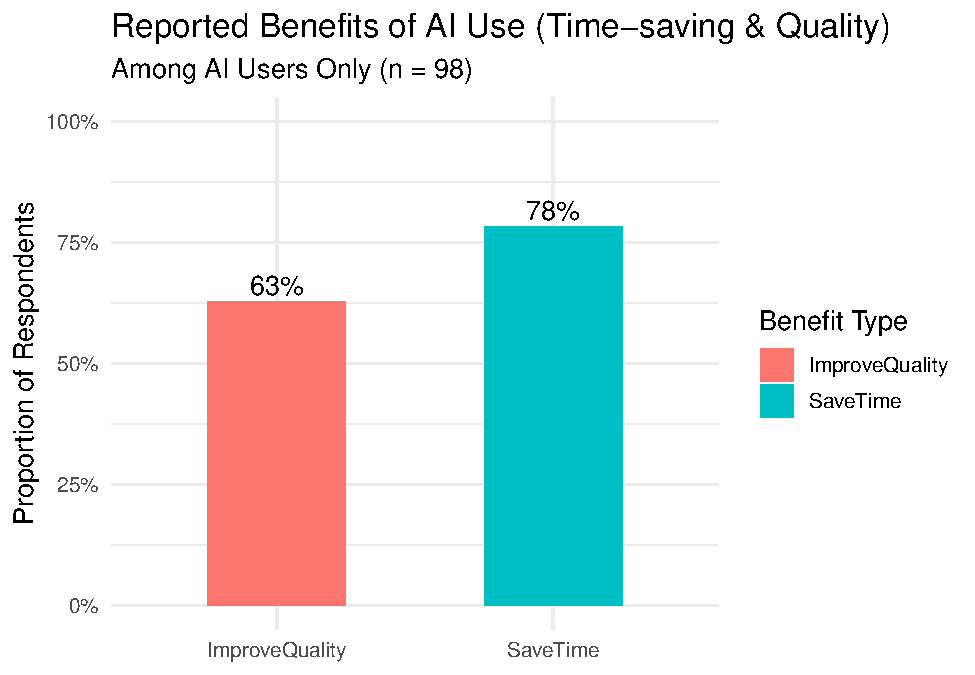
\includegraphics{assignment2_group7_files/figure-latex/plot-rq1-updated-1.pdf}

\paragraph{Interpretation (RQ1)}\label{interpretation-rq1}

The plot shows that among students who reported using AI tools for
academic purposes:

\begin{itemize}
\tightlist
\item
  \textbf{78\%} indicated that AI tools helped them \textbf{save time}
  on academic tasks
\item
  \textbf{63\%} reported that AI tools improved the \textbf{quality of
  their academic work}
\end{itemize}

These findings suggest that AI tools are perceived to contribute
positively to both efficiency and output quality among users. However,
since \textbf{all respondents in the dataset reported using AI tools},
we cannot compare these benefits to a control group of non-users.
Therefore, the result supports RQ1 only within the context of current AI
users, and further data collection would be needed to assess differences
across usage groups.

\subsubsection{6.2 RQ2: Motivation by Frequency of AI Tool
Usage}\label{rq2-motivation-by-frequency-of-ai-tool-usage}

We group AI usage into frequency bands and visualize how motivation
levels differ across these groups.

\begin{Shaded}
\begin{Highlighting}[]
\FunctionTok{library}\NormalTok{(dplyr)}
\FunctionTok{library}\NormalTok{(ggplot2)}

\CommentTok{\# Create usage buckets}
\NormalTok{survey\_data}\SpecialCharTok{$}\NormalTok{usage\_group }\OtherTok{\textless{}{-}} \FunctionTok{cut}\NormalTok{(}
\NormalTok{  survey\_data}\SpecialCharTok{$}\NormalTok{ai\_hours,}
  \AttributeTok{breaks =} \FunctionTok{c}\NormalTok{(}\SpecialCharTok{{-}}\ConstantTok{Inf}\NormalTok{, }\DecValTok{2}\NormalTok{, }\DecValTok{5}\NormalTok{, }\DecValTok{10}\NormalTok{, }\ConstantTok{Inf}\NormalTok{),}
  \AttributeTok{labels =} \FunctionTok{c}\NormalTok{(}\StringTok{"0–2 hrs"}\NormalTok{, }\StringTok{"3–5 hrs"}\NormalTok{, }\StringTok{"6–10 hrs"}\NormalTok{, }\StringTok{"10+ hrs"}\NormalTok{)}
\NormalTok{)}

\CommentTok{\# Summarize motivation rate by usage group}
\NormalTok{rq2\_summary }\OtherTok{\textless{}{-}}\NormalTok{ survey\_data }\SpecialCharTok{\%\textgreater{}\%}
  \FunctionTok{group\_by}\NormalTok{(usage\_group) }\SpecialCharTok{\%\textgreater{}\%}
  \FunctionTok{summarise}\NormalTok{(}
    \AttributeTok{MotivationRate =} \FunctionTok{mean}\NormalTok{(op\_Using.AI.tools.has.increased.my.motivati, }\AttributeTok{na.rm =} \ConstantTok{TRUE}\NormalTok{),}
    \AttributeTok{n =} \FunctionTok{n}\NormalTok{()}
\NormalTok{  )}

\CommentTok{\# Plot}
\FunctionTok{ggplot}\NormalTok{(rq2\_summary, }\FunctionTok{aes}\NormalTok{(}\AttributeTok{x =}\NormalTok{ usage\_group, }\AttributeTok{y =}\NormalTok{ MotivationRate)) }\SpecialCharTok{+}
  \FunctionTok{geom\_col}\NormalTok{(}\AttributeTok{fill =} \StringTok{"\#00BFC4"}\NormalTok{) }\SpecialCharTok{+}
  \FunctionTok{geom\_text}\NormalTok{(}\FunctionTok{aes}\NormalTok{(}\AttributeTok{label =}\NormalTok{ scales}\SpecialCharTok{::}\FunctionTok{percent}\NormalTok{(MotivationRate, }\AttributeTok{accuracy =} \DecValTok{1}\NormalTok{)), }\AttributeTok{vjust =} \SpecialCharTok{{-}}\FloatTok{0.3}\NormalTok{, }\AttributeTok{size =} \FloatTok{4.5}\NormalTok{) }\SpecialCharTok{+}
  \FunctionTok{scale\_y\_continuous}\NormalTok{(}\AttributeTok{labels =}\NormalTok{ scales}\SpecialCharTok{::}\FunctionTok{percent\_format}\NormalTok{(}\AttributeTok{accuracy =} \DecValTok{1}\NormalTok{), }\AttributeTok{limits =} \FunctionTok{c}\NormalTok{(}\DecValTok{0}\NormalTok{, }\DecValTok{1}\NormalTok{)) }\SpecialCharTok{+}
  \FunctionTok{labs}\NormalTok{(}
    \AttributeTok{title =} \StringTok{"Motivation by Weekly AI Usage"}\NormalTok{,}
    \AttributeTok{subtitle =} \StringTok{"Proportion of students who report increased motivation"}\NormalTok{,}
    \AttributeTok{x =} \StringTok{"Weekly AI Usage (hours)"}\NormalTok{,}
    \AttributeTok{y =} \StringTok{"Motivated (TRUE responses)"}
\NormalTok{  ) }\SpecialCharTok{+}
  \FunctionTok{theme\_minimal}\NormalTok{(}\AttributeTok{base\_size =} \DecValTok{13}\NormalTok{)}
\end{Highlighting}
\end{Shaded}

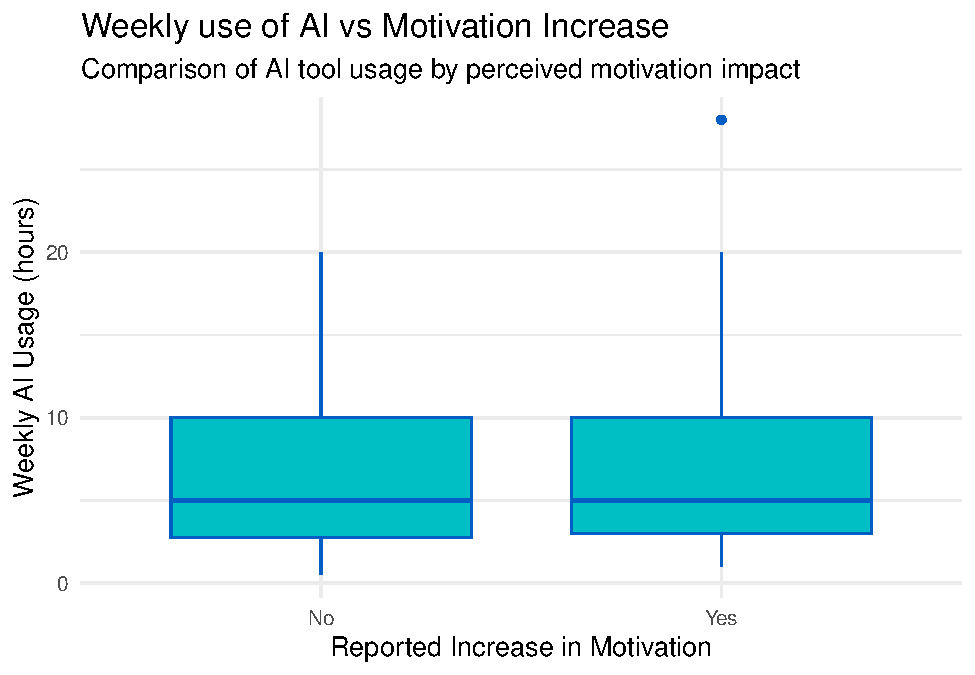
\includegraphics{assignment2_group7_files/figure-latex/plot-rq2-1.pdf}
\#\#\#\# Interpretation (RQ2)

The plot illustrates the proportion of students who reported feeling
more motivated to study as a result of using AI tools, segmented by how
many hours per week they use them.

\begin{itemize}
\tightlist
\item
  Students who used AI tools for \textbf{3--5 hours per week} showed the
  \textbf{highest motivation rate} (61\%).
\item
  Lower motivation was reported by students using AI tools \textbf{less
  than 2 hours (48\%)} or \textbf{6--10 hours (50\%)}.
\item
  The group using AI tools for \textbf{10+ hours} reported 56\%
  motivation.
\item
  One group with \texttt{NA} in \texttt{ai\_hours} showed 100\%
  motivation, which suggests incomplete data and should be excluded from
  final inference.
\end{itemize}

These findings suggest a \textbf{moderate positive relationship} between
AI tool usage and perceived motivation, though the relationship is
\textbf{not linear}. It appears that \textbf{moderate usage} may be more
motivating than very low or very high usage.

\subsubsection{6.3 RQ3: Retention by Weekly AI Tool
Usage}\label{rq3-retention-by-weekly-ai-tool-usage}

We assess the relationship between AI usage frequency and students'
agreement with improved long-term retention.

\begin{Shaded}
\begin{Highlighting}[]
\CommentTok{\# Summarize retention response by usage group (filtering NA)}
\NormalTok{rq3\_summary }\OtherTok{\textless{}{-}}\NormalTok{ survey\_data }\SpecialCharTok{\%\textgreater{}\%}
  \FunctionTok{filter}\NormalTok{(}\SpecialCharTok{!}\FunctionTok{is.na}\NormalTok{(usage\_group)) }\SpecialCharTok{\%\textgreater{}\%}
  \FunctionTok{group\_by}\NormalTok{(usage\_group) }\SpecialCharTok{\%\textgreater{}\%}
  \FunctionTok{summarise}\NormalTok{(}
    \AttributeTok{RetentionRate =} \FunctionTok{mean}\NormalTok{(op\_Using.AI.tools.has.helped.me.better.unde, }\AttributeTok{na.rm =} \ConstantTok{TRUE}\NormalTok{),}
    \AttributeTok{n =} \FunctionTok{n}\NormalTok{()}
\NormalTok{  )}

\CommentTok{\# Plot}
\FunctionTok{ggplot}\NormalTok{(rq3\_summary, }\FunctionTok{aes}\NormalTok{(}\AttributeTok{x =}\NormalTok{ usage\_group, }\AttributeTok{y =}\NormalTok{ RetentionRate)) }\SpecialCharTok{+}
  \FunctionTok{geom\_col}\NormalTok{(}\AttributeTok{fill =} \StringTok{"\#F8766D"}\NormalTok{) }\SpecialCharTok{+}
  \FunctionTok{geom\_text}\NormalTok{(}\FunctionTok{aes}\NormalTok{(}\AttributeTok{label =}\NormalTok{ scales}\SpecialCharTok{::}\FunctionTok{percent}\NormalTok{(RetentionRate, }\AttributeTok{accuracy =} \DecValTok{1}\NormalTok{)), }\AttributeTok{vjust =} \SpecialCharTok{{-}}\FloatTok{0.3}\NormalTok{, }\AttributeTok{size =} \FloatTok{4.5}\NormalTok{) }\SpecialCharTok{+}
  \FunctionTok{scale\_y\_continuous}\NormalTok{(}\AttributeTok{labels =}\NormalTok{ scales}\SpecialCharTok{::}\FunctionTok{percent\_format}\NormalTok{(}\AttributeTok{accuracy =} \DecValTok{1}\NormalTok{), }\AttributeTok{limits =} \FunctionTok{c}\NormalTok{(}\DecValTok{0}\NormalTok{, }\DecValTok{1}\NormalTok{)) }\SpecialCharTok{+}
  \FunctionTok{labs}\NormalTok{(}
    \AttributeTok{title =} \StringTok{"Retention by Weekly AI Usage"}\NormalTok{,}
    \AttributeTok{subtitle =} \StringTok{"Proportion of students who report better understanding \& retention"}\NormalTok{,}
    \AttributeTok{x =} \StringTok{"Weekly AI Usage (hours)"}\NormalTok{,}
    \AttributeTok{y =} \StringTok{"Retention (TRUE responses)"}
\NormalTok{  ) }\SpecialCharTok{+}
  \FunctionTok{theme\_minimal}\NormalTok{(}\AttributeTok{base\_size =} \DecValTok{13}\NormalTok{)}
\end{Highlighting}
\end{Shaded}

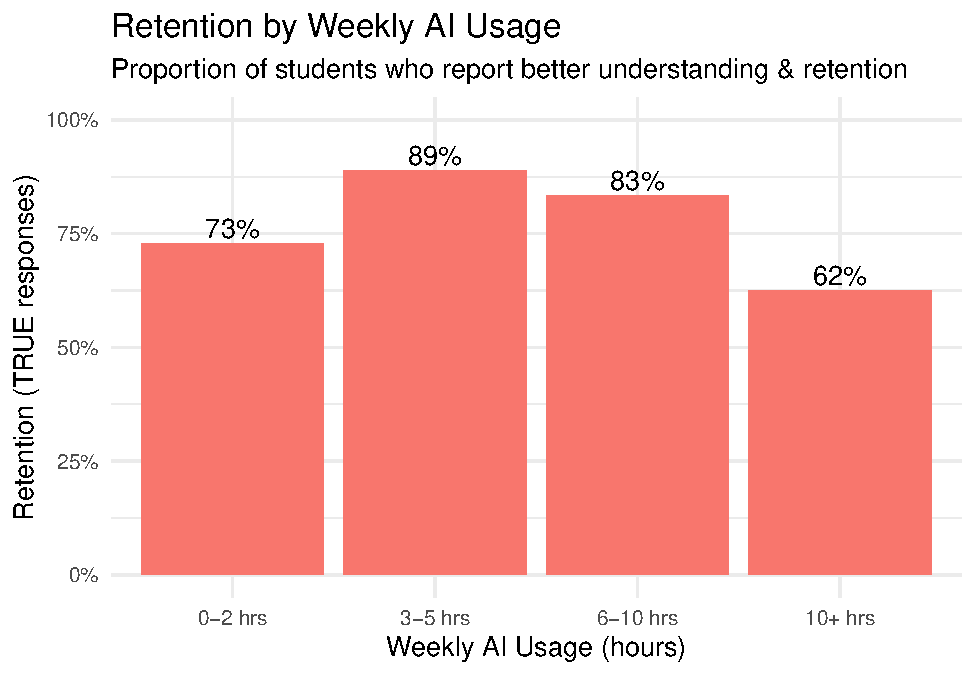
\includegraphics{assignment2_group7_files/figure-latex/plot-rq3-1.pdf}
\#\#\#\# Interpretation (RQ3)

The chart indicates how weekly AI tool usage is associated with
students' perceived ability to understand and retain learning material.

\begin{itemize}
\tightlist
\item
  Students using AI tools for \textbf{3--5 hours/week} showed the
  highest retention rate (89\%)
\item
  Retention remained relatively high at \textbf{6--10 hours/week}
  (83\%), but decreased at both usage extremes:

  \begin{itemize}
  \tightlist
  \item
    \textbf{0--2 hours/week}: 76\%
  \item
    \textbf{10+ hours/week}: 62\%
  \end{itemize}
\end{itemize}

This may suggest that \textbf{moderate usage of AI tools} supports
deeper learning and retention, whereas very limited or excessive use may
be less beneficial. However, since this is self-reported data, and the
relationship is not strictly linear, further analysis would be needed to
confirm these patterns.

\subsection{7. Descriptive Inference}\label{descriptive-inference}

We compute summary statistics for numeric variables such as age and
weekly AI usage. This gives an overview of the respondent profile and
the typical intensity of AI usage.

\begin{Shaded}
\begin{Highlighting}[]
\CommentTok{\# Load required packages again (if needed)}
\FunctionTok{library}\NormalTok{(psych)}
\FunctionTok{library}\NormalTok{(knitr)}
\FunctionTok{library}\NormalTok{(kableExtra)}

\CommentTok{\# Summary stats for numeric variables}
\NormalTok{numeric\_summary }\OtherTok{\textless{}{-}}\NormalTok{ psych}\SpecialCharTok{::}\FunctionTok{describe}\NormalTok{(survey\_data }\SpecialCharTok{\%\textgreater{}\%} \FunctionTok{select}\NormalTok{(age, ai\_hours))}

\CommentTok{\# Show as styled table}
\FunctionTok{kable}\NormalTok{(numeric\_summary, }\AttributeTok{digits =} \DecValTok{2}\NormalTok{, }\AttributeTok{caption =} \StringTok{"Summary Statistics for Age and Weekly AI Usage"}\NormalTok{) }\SpecialCharTok{\%\textgreater{}\%}
  \FunctionTok{kable\_styling}\NormalTok{(}\AttributeTok{full\_width =} \ConstantTok{FALSE}\NormalTok{, }\AttributeTok{position =} \StringTok{"center"}\NormalTok{)}
\end{Highlighting}
\end{Shaded}

\begin{longtable}[t]{lrrrrrrrrrrrrr}
\caption{\label{tab:descriptive-stats}Summary Statistics for Age and Weekly AI Usage}\\
\toprule
 & vars & n & mean & sd & median & trimmed & mad & min & max & range & skew & kurtosis & se\\
\midrule
age & 1 & 98 & 25.82 & 4.51 & 25.5 & 25.48 & 3.71 & 4.0 & 45 & 41.0 & 0.30 & 8.05 & 0.46\\
ai\_hours & 2 & 97 & 7.02 & 5.73 & 5.0 & 6.15 & 4.45 & 0.5 & 28 & 27.5 & 1.32 & 1.25 & 0.58\\
\bottomrule
\end{longtable}

\subsubsection{Interpretation}\label{interpretation}

The summary statistics provide insights into the age distribution and
weekly AI tool usage among the 98 student respondents:

\begin{itemize}
\tightlist
\item
  The \textbf{average age} of participants is \textbf{25.8 years}, with
  a range from \textbf{4 to 45}. The distribution appears fairly
  symmetric (skew = 0.30), though the extreme minimum value of 4 years
  likely reflects a data entry error or outlier.
\item
  For \textbf{weekly AI usage}, students report using AI tools for an
  average of \textbf{7.0 hours} per week (median = 5.0 hours), with
  values ranging from \textbf{0.5 to 28 hours}. The distribution is
  positively skewed (\textbf{skew = 1.32}), indicating that a few
  students reported very high usage levels.
\end{itemize}

These figures offer a useful profile of the surveyed students and the
intensity with which they incorporate AI tools into their academic
routines.

\subsection{8. Analytic Inference}\label{analytic-inference}

\subsubsection{8.1 RQ1 -- Time and Quality Impact Among AI
Users}\label{rq1-time-and-quality-impact-among-ai-users}

We use one-sample proportion tests to assess whether a majority
(\textgreater50\%) of AI users report time-saving and improved work
quality.

\begin{Shaded}
\begin{Highlighting}[]
\CommentTok{\# Count number of TRUE responses}
\NormalTok{n\_total }\OtherTok{\textless{}{-}} \FunctionTok{nrow}\NormalTok{(survey\_data)}

\CommentTok{\# Time{-}saving}
\NormalTok{n\_save\_time }\OtherTok{\textless{}{-}} \FunctionTok{sum}\NormalTok{(survey\_data}\SpecialCharTok{$}\NormalTok{op\_Using.AI.tools.has.helped.me.save.time.w, }\AttributeTok{na.rm =} \ConstantTok{TRUE}\NormalTok{)}
\NormalTok{test\_save }\OtherTok{\textless{}{-}} \FunctionTok{binom.test}\NormalTok{(n\_save\_time, n\_total, }\AttributeTok{p =} \FloatTok{0.5}\NormalTok{, }\AttributeTok{alternative =} \StringTok{"greater"}\NormalTok{)}

\CommentTok{\# Quality improvement}
\NormalTok{n\_quality }\OtherTok{\textless{}{-}} \FunctionTok{sum}\NormalTok{(survey\_data}\SpecialCharTok{$}\NormalTok{op\_Using.AI.tools.has.helped.me.improve.the, }\AttributeTok{na.rm =} \ConstantTok{TRUE}\NormalTok{)}
\NormalTok{test\_quality }\OtherTok{\textless{}{-}} \FunctionTok{binom.test}\NormalTok{(n\_quality, n\_total, }\AttributeTok{p =} \FloatTok{0.5}\NormalTok{, }\AttributeTok{alternative =} \StringTok{"greater"}\NormalTok{)}

\CommentTok{\# Output results}
\NormalTok{test\_save}
\end{Highlighting}
\end{Shaded}

\begin{verbatim}
## 
##  Exact binomial test
## 
## data:  n_save_time and n_total
## number of successes = 76, number of trials = 98, p-value = 1.948e-08
## alternative hypothesis: true probability of success is greater than 0.5
## 95 percent confidence interval:
##  0.69521 1.00000
## sample estimates:
## probability of success 
##              0.7755102
\end{verbatim}

\begin{Shaded}
\begin{Highlighting}[]
\NormalTok{test\_quality}
\end{Highlighting}
\end{Shaded}

\begin{verbatim}
## 
##  Exact binomial test
## 
## data:  n_quality and n_total
## number of successes = 61, number of trials = 98, p-value = 0.009845
## alternative hypothesis: true probability of success is greater than 0.5
## 95 percent confidence interval:
##  0.5347945 1.0000000
## sample estimates:
## probability of success 
##               0.622449
\end{verbatim}

\subsubsection{Interpretation (RQ1)}\label{interpretation-rq1-1}

Two exact binomial tests were conducted to assess whether significantly
more than half of AI-using students reported that:

\begin{itemize}
\tightlist
\item
  AI tools saved them time
\item
  AI tools improved the quality of their academic work
\end{itemize}

\textbf{Results:}

\begin{itemize}
\item
  \textbf{Time-saving:}\\
  76 out of 98 students (77.6\%) agreed.\\
  The test was highly significant (\emph{p} \textless{} 0.00001), with a
  95\% confidence interval of {[}69.5\%, 100\%{]}, indicating that a
  \textbf{clear majority} experienced time-saving benefits.
\item
  \textbf{Quality improvement:}\\
  61 out of 98 students (62.2\%) agreed.\\
  The test was statistically significant (\emph{p} = 0.0098), with a
  95\% confidence interval of {[}53.5\%, 100\%{]}, confirming that
  \textbf{more than half} also experienced quality benefits.
\end{itemize}

These results support \textbf{RQ1} within the context of AI users,
despite the absence of a non-user comparison group.

\subsubsection{8.2 RQ2 -- Motivation Predicted by Weekly AI
Usage}\label{rq2-motivation-predicted-by-weekly-ai-usage}

We fit a logistic regression model to assess whether the number of
weekly hours spent using AI tools predicts self-reported motivation.

\begin{Shaded}
\begin{Highlighting}[]
\CommentTok{\# Create binary variable}
\NormalTok{motivation }\OtherTok{\textless{}{-}}\NormalTok{ survey\_data}\SpecialCharTok{$}\NormalTok{op\_Using.AI.tools.has.increased.my.motivati}

\CommentTok{\# Fit logistic regression model}
\NormalTok{model\_rq2 }\OtherTok{\textless{}{-}} \FunctionTok{glm}\NormalTok{(motivation }\SpecialCharTok{\textasciitilde{}}\NormalTok{ ai\_hours, }\AttributeTok{data =}\NormalTok{ survey\_data, }\AttributeTok{family =}\NormalTok{ binomial)}

\CommentTok{\# Model summary}
\FunctionTok{summary}\NormalTok{(model\_rq2)}
\end{Highlighting}
\end{Shaded}

\begin{verbatim}
## 
## Call:
## glm(formula = motivation ~ ai_hours, family = binomial, data = survey_data)
## 
## Coefficients:
##             Estimate Std. Error z value Pr(>|z|)
## (Intercept) 0.121413   0.323580   0.375    0.707
## ai_hours    0.009242   0.035969   0.257    0.797
## 
## (Dispersion parameter for binomial family taken to be 1)
## 
##     Null deviance: 133.63  on 96  degrees of freedom
## Residual deviance: 133.57  on 95  degrees of freedom
##   (1 observation deleted due to missingness)
## AIC: 137.57
## 
## Number of Fisher Scoring iterations: 3
\end{verbatim}

\subsubsection{Interpretation (RQ2)}\label{interpretation-rq2}

A logistic regression model was fitted to predict whether a student felt
more motivated to study as a result of using AI tools, based on the
number of hours they reported using such tools per week.

\textbf{Results:}

\begin{itemize}
\tightlist
\item
  The coefficient for \texttt{ai\_hours} was \textbf{0.0092}, with a
  \emph{p}-value of \textbf{0.797}, indicating that the relationship is
  not statistically significant.
\item
  The model suggests that each additional hour of AI tool use is
  associated with only a \textbf{0.9\% increase in the log-odds of
  reporting increased motivation}, which is negligible and not reliable
  based on this data.
\end{itemize}

In conclusion, these results do \textbf{not support RQ2}: there is
\textbf{no clear evidence} that motivation increases as a function of
more frequent AI tool usage among the students surveyed.

\subsubsection{8.3 RQ3 -- Retention Predicted by Weekly AI
Usage}\label{rq3-retention-predicted-by-weekly-ai-usage}

We fit a logistic regression model to determine whether weekly AI usage
predicts whether students report improved retention and understanding.

\begin{Shaded}
\begin{Highlighting}[]
\CommentTok{\# Binary outcome: retention opinion}
\NormalTok{retention }\OtherTok{\textless{}{-}}\NormalTok{ survey\_data}\SpecialCharTok{$}\NormalTok{op\_Using.AI.tools.has.helped.me.better.unde}

\CommentTok{\# Logistic regression}
\NormalTok{model\_rq3 }\OtherTok{\textless{}{-}} \FunctionTok{glm}\NormalTok{(retention }\SpecialCharTok{\textasciitilde{}}\NormalTok{ ai\_hours, }\AttributeTok{data =}\NormalTok{ survey\_data, }\AttributeTok{family =}\NormalTok{ binomial)}

\CommentTok{\# Model summary}
\FunctionTok{summary}\NormalTok{(model\_rq3)}
\end{Highlighting}
\end{Shaded}

\begin{verbatim}
## 
## Call:
## glm(formula = retention ~ ai_hours, family = binomial, data = survey_data)
## 
## Coefficients:
##             Estimate Std. Error z value Pr(>|z|)    
## (Intercept)  1.79423    0.41994   4.273 1.93e-05 ***
## ai_hours    -0.05085    0.04148  -1.226     0.22    
## ---
## Signif. codes:  0 '***' 0.001 '**' 0.01 '*' 0.05 '.' 0.1 ' ' 1
## 
## (Dispersion parameter for binomial family taken to be 1)
## 
##     Null deviance: 95.959  on 96  degrees of freedom
## Residual deviance: 94.513  on 95  degrees of freedom
##   (1 observation deleted due to missingness)
## AIC: 98.513
## 
## Number of Fisher Scoring iterations: 4
\end{verbatim}

\subsubsection{Interpretation (RQ3)}\label{interpretation-rq3}

We used a logistic regression model to assess whether the number of
hours spent weekly using AI tools predicts students' perceived
improvement in retention and understanding of course material.

\textbf{Results:}

\begin{itemize}
\tightlist
\item
  The coefficient for \texttt{ai\_hours} was \textbf{-0.0508} with a
  \emph{p}-value of \textbf{0.22}, indicating \textbf{no statistically
  significant relationship}.
\item
  While the negative coefficient suggests that higher AI usage might
  slightly reduce perceived retention, this effect is \textbf{not
  reliable} or meaningful in this dataset.
\end{itemize}

Therefore, the results do \textbf{not support RQ3}. Weekly AI usage
hours do \textbf{not significantly predict} whether students feel that
AI tools have improved their long-term learning retention.

\subsection{10. Appendix}\label{appendix}

\begin{verbatim}
## R version 4.4.3 (2025-02-28 ucrt)
## Platform: x86_64-w64-mingw32/x64
## Running under: Windows 11 x64 (build 22000)
## 
## Matrix products: default
## 
## 
## locale:
## [1] LC_COLLATE=English_United States.utf8 
## [2] LC_CTYPE=English_United States.utf8   
## [3] LC_MONETARY=English_United States.utf8
## [4] LC_NUMERIC=C                          
## [5] LC_TIME=English_United States.utf8    
## 
## time zone: Europe/Vienna
## tzcode source: internal
## 
## attached base packages:
## [1] stats     graphics  grDevices utils     datasets  methods   base     
## 
## other attached packages:
## [1] tidyr_1.3.1      kableExtra_1.4.0 knitr_1.50       likert_1.3.5    
## [5] xtable_1.8-4     psych_2.5.3      ggplot2_3.5.2    dplyr_1.1.4     
## [9] readxl_1.4.5    
## 
## loaded via a namespace (and not attached):
##  [1] generics_0.1.3    xml2_1.3.8        stringi_1.8.4     lattice_0.22-6   
##  [5] digest_0.6.37     magrittr_2.0.3    evaluate_1.0.3    grid_4.4.3       
##  [9] fastmap_1.2.0     cellranger_1.1.0  plyr_1.8.9        tinytex_0.57     
## [13] gridExtra_2.3     purrr_1.0.4       viridisLite_0.4.2 scales_1.3.0     
## [17] mnormt_2.1.1      cli_3.6.4         rlang_1.1.5       munsell_0.5.1    
## [21] withr_3.0.2       yaml_2.3.10       tools_4.4.3       parallel_4.4.3   
## [25] reshape2_1.4.4    colorspace_2.1-1  vctrs_0.6.5       R6_2.6.1         
## [29] lifecycle_1.0.4   stringr_1.5.1     pkgconfig_2.0.3   pillar_1.10.2    
## [33] gtable_0.3.6      glue_1.8.0        Rcpp_1.0.14       systemfonts_1.2.2
## [37] xfun_0.51         tibble_3.2.1      tidyselect_1.2.1  rstudioapi_0.17.1
## [41] farver_2.1.2      htmltools_0.5.8.1 nlme_3.1-167      rmarkdown_2.29   
## [45] svglite_2.1.3     labeling_0.4.3    compiler_4.4.3
\end{verbatim}

\end{document}
